\documentclass{modeleRapport}

\bibliography{biblio.bib}
\usepackage{lmodern}
\usepackage{listings}
\lstset{
    numbers=none,   % No line numbers
    frame=none,     % No frame around the code
    basicstyle=\ttfamily, % Use a monospace font
    language=Python  % Specify the language for syntax highlighting
}
\hbadness=10000
\vbadness=10000
\scrollmode % Send warning to logs not to show them upon compiling

%--------------------------------------

\titre{Machine Learning Project}
\soustitre{ESILV A4 - DIA2}

\enseignant{Nédra \textsc{MELLOULI} \\
            Zachary \textsc{FAKIR} }

\eleves{Nour \textsc{AFFES} \\
	Lucas \textsc{BLANCHET} \\ 
	Hugo \textsc{BONNELL} \\
    Rayan \textsc{HAMADEH}}

%--------------------------------------

\begin{document}

\fairepagedegarde
\fairetabledesmatieres

%--------------------------------------

\section{Problem Overview}

\subsection{Problem Definition}

Drowsy driving, a serious hazard often resulting from insufficient rest, causes drivers to lose focus, 
react more slowly, and even experience brief micro-sleeps. This issue has devastating impacts, contributing to 
approximately 328,000 accidents, 109,000 injuries, and 6,400 fatalities annually (Bankrate \cite{Bankrate}). 
Unlike the effects of alcohol or drugs, drowsiness is harder to detect, creating a challenge for preventive measures. 
A 2019 AAA Foundation \cite{AAAFoundation} study reveals that while 96\% of drivers recognize the extreme risk of drowsy 
driving, only 29\% feel that they are at risk of getting pulled over by law enforcement. 


\subsubsection{Existing technologies}

\begin{itemize}
\item \textbf{Mercedes-Benz ATTENTION ASSIST} \cite{Mercedes}: analyzes driving pattern in the first few minutes of the 
ride, and then detects patterns that might be due to fatigue, and alerts by a coffee cup symbol on the dashboard.  

\item F\textbf{ord Driver Alert System} \cite{Ford}: monitor level of alertness based on driving behavior, an alert is 
displayed on the information display, that will be automatically cleared after a while and can also be cleared by pressing 
ok on the steering wheel. This feature can be turned off and will stay off even if you turn the ignition off and back on. 
This method can be impacted by windshield conditions such as bird droppings, ice, or snow. System is only available at speeds 
below activation speed (64 km/h) Proposed Solution and Business Objectives. 
\end{itemize}

Our project aims to develop a machine-learning-powered system that monitors driver fatigue in real-time. This solution will leverage a camera-based approach, ideally suited to modern vehicles already equipped with interior cameras. Unlike current technology, this model will focus directly on the driver’s condition by analyzing eye and mouth states, reducing dependence on external driving conditions. 

\subsubsection{Key business objectives}

\begin{itemize}

\item \textbf{Increase Road Safety :} By alerting drivers when drowsiness indicators are detected, the system can help prevent accidents. 

\item \textbf{Enhance Detection Accuracy :} Monitoring eye and mouth states ensures fatigue detection remains consistent across different road, traffic, and weather conditions. 

\item \textbf{Offer a Scalable Solution :} Using a straightforward dataset and CNN model, the system is designed to integrate smoothly into existing vehicle technology, avoiding significant production costs. 

\item \textbf{Foundation for Advanced Safety Features :} In future applications, the model could work with autonomous driving technology to execute actions like parking assistance or alerting emergency services if the driver fails to respond. 

\end{itemize}

\subsection{Dataset Description}

The dataset \cite{Dataset} for this project contains labeled images indicating whether a driver’s eyes are “open” or “closed” and mouth states as “yawn” or “no yawn.” This binary classification structure aligns well with a CNN model, allowing us to detect drowsiness through simple yet reliable features, focusing on real-time driver monitoring. By building a robust CNN on this well-labeled dataset, we emphasize a driver-centric approach, which addresses existing technology gaps in driver fatigue detection. 

\subsection{Scope}

The scope of this project covers the development, testing, and evaluation of a computer vision-based drowsiness detection model. Key components include: 

\begin{itemize}

\item \textbf{Model Development :} Implementing a Convolutional Neural Network (CNN) to accurately classify eye and mouth states from real-time image data. These classifications will enable reliable identification of closed eyes or yawning—critical indicators of drowsiness. 

\item \textbf{Real-Time Deployment Potential :} Optimizing the model architecture to minimize latency, with potential for integration into embedded vehicle systems. 

\item \textbf{Driver-Centric Focus :} The model will monitor the driver’s physical state, making it adaptable to various driving environments, road types, and vehicle models. 

\item \textbf{Alert System :} Although primary development focuses on detection accuracy, we will outline alert system recommendations to ensure the notifications are clear and hard to ignore for drowsy drivers. 

\end{itemize}

\subsection{Organization}

A structured Gantt chart outlines each phase of this project, helping to ensure timely and organized progression. The tasks are divided into four major phases: Implementing a standard solution, improving it for stage 2, further improvements for stage 3 and finally, Report and Presentation Preparation. Each task is designed with inter-dependencies in mind, ensuring a streamlined workflow and timely completion of project milestones.

%---------------------------------------
\newpage

\section{Preparing the Data and the Analysis}

\subsection{Problem Formalization}
\subsubsection{Problem Statement}
The primary objective here is to develop a machine-learning-powered system that monitors driver fatigue in real-time. This model will focus directly on the driver’s condition by analyzing eye and mouth states and deduce if the driver is in a tired state accurately.
\subsubsection{Understanding the Dataset}
As we said before, our dataset consists of labeled images indicating whether a driver’s eyes are “open” or “closed” and mouth states as “yawn” or “no yawn.” The data is balanced: we have the same distribution between classes (726 for both closed and open and 723/725 for yawn and no yawn respectively) so we won’t have an issue with biased model prediction or poor performance on minority class. \\

\textbf{Dataset Overview:}
\begin{table}[H]
    \centering
    \begin{tabular}{|c|c|c|c|}
        \hline
        Eye Closed & Eye Opened & Mouth Yawn & Mouth no Yawn \\
        \hline
        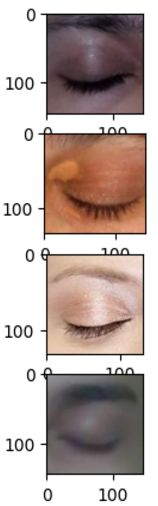
\includegraphics[width=3cm]{Images/eyeClosed.png}
        &
        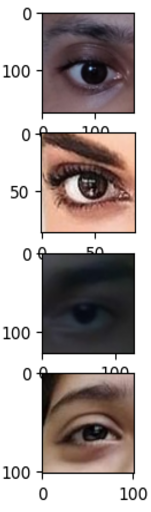
\includegraphics[width=3cm]{Images/eyeOpen.png}
        &
        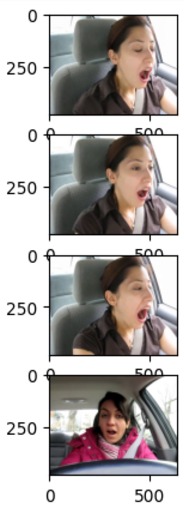
\includegraphics[width=3cm]{Images/yawn.png}
        &
        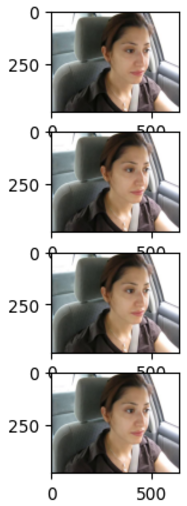
\includegraphics[width=3cm]{Images/noYawn.png}
        \\
        \hline
    \end{tabular}
    \caption{Examples of images per label.}
\end{table}

\newpage
\textbf{Data Characteristics:}
\begin{itemize}
    \item Our dataset is made of images. Each image can be represented as a matrix. Each value in this matrix is an array with the RGB values of the corresponding pixel.
    \item The images in our dataset don't share the same dimensions. This may yield unexpected results after training models on this data. Thus, we'll have to handle image formatting before doing any train.\\
\end{itemize}

\textbf{Model goals:}
\begin{itemize}
    \item \textbf{Primary objective :} 
    \begin{itemize}
        \item Being able to tell if a driver is showing tireness symptoms.
    \end{itemize}
    \item \textbf{Secondary objectives :}
    \begin{itemize}
        \item Ensure our model is robust.
        \item Ensure the model can handle a variety of data inputs by not over-fitting.
    \end{itemize}
\end{itemize}

\subsection{Refining the Dataset}
Our initial task involved meticulously cleaning and pre-processing the data. This process was crucial to ensure the integrity and usability of the dataset for machine learning models. Key steps included: 
\begin{itemize}
    \item To handle missing or corrupted values.
    \item To remove duplicates if any.
    \item To make sure that all pictures have the same size.
\end{itemize}

\subsection{Evaluation Metrics}

\begin{itemize}
    \item In addition to \textbf{accuracy}, we considered other metrics like \textbf{precision, recall, and F1 score} for a comprehensive assessment of our models. These metrics provided a more nuanced view of the model's performance because we need to be as accurate as possible. 
    \item We'll also use \textbf{Confusion Matrices} as a mean of better understanding the results of the models we're testing.
\end{itemize}

\subsection{Data cleaning and pre-processing}

In the process of preparing our data for our machine learning project, our group followed a set of essential steps.

\begin{codebox}[Data cleaning]{Checking for missing or corrupted data \texttt{Python}}
\begin{lstlisting}
from PIL import Image
import os

def count_corrupted_images(dataset_path):
    corrupted_count = 0
    total_images = 0

    for root, _, files in os.walk(dataset_path):
        for file in files:
            file_path = os.path.join(root, file)
            total_images += 1
            try:
                with Image.open(file_path) as img:
                    img.verify()
            except Exception as e:
                corrupted_count += 1
                print(f"Corrupted: {file_path} - Error: {e}")

    print(f"\nTotal Images Checked: {total_images}")
    print(f"Total Corrupted Images: {corrupted_count}")
    return corrupted_count

count_corrupted_images(path+"/train/Closed")
count_corrupted_images(path+"/train/Open")
count_corrupted_images(path+"/train/yawn")
count_corrupted_images(path+"/train/no_yawn")
\end{lstlisting}
\end{codebox}

\begin{codebox}[OutputA]{ Output of Code 1}
Total Images Checked: 726\\
Total Corrupted Images: 0\\
\\
Total Images Checked: 726\\
Total Corrupted Images: 0\\
\\
Total Images Checked: 723\\
Total Corrupted Images: 0\\
\\
Total Images Checked: 725\\
Total Corrupted Images: 0\\
\end{codebox}

We don't have any corrputed file in the dataset. Let's check for duplicates:

\begin{codebox}[Duplicate Check]{Checking for duplicate data \texttt{Python}}
\begin{lstlisting}
import hashlib
import cv2
import os

def remove_duplicates(dataset_path):
    image_hashes = {}
    unique_images = []

    for root, _, files in os.walk(dataset_path):  
        for file in files:
            file_path = os.path.join(root, file)  

            img = cv2.imread(file_path, cv2.IMREAD_GRAYSCALE)

            img_bytes = img.tobytes()

            img_hash = hashlib.md5(img_bytes).hexdigest()

            if img_hash not in image_hashes:
                image_hashes[img_hash] = file_path
                unique_images.append(file_path)
            else:
                return(f"Duplicate found: {file_path}")

    return ("There are no duplicate images")


remove_duplicates(path + "/train/Closed")
remove_duplicates(path + "/train/Open")
remove_duplicates(path + "/train/yawn")
remove_duplicates(path + "/train/no_yawn")
\end{lstlisting}
\end{codebox}

\begin{codebox}[OutputB]{ Output of Code 3}
'There are no duplicate images'
\end{codebox}

As stated in Code 4, the pictures are all unique, we can use all of them.
\newpage
Finally, we will use some pre-processing techniques such as:\\
\begin{itemize}

\item \textbf{Image Transformation} to make all the image have the same size and increases the accuracy.\\

\begin{codebox}[Image Transformation]{Image transformation - resize images \texttt{Python}}
\begin{lstlisting}
def load_images(dataset_path, target_size=(64, 64)):
    images = []
    labels = []
    for label in os.listdir(dataset_path):
        class_path = os.path.join(dataset_path, label)
        if not os.path.isdir(class_path):
            continue
        for img_file in os.listdir(class_path):
            img_path = os.path.join(class_path, img_file)
            img = cv2.imread(img_path, cv2.IMREAD_GRAYSCALE) 
            if img is not None:
                img_resized = cv2.resize(img, target_size) 
                images.append(img_resized.flatten())
                labels.append(label)
    return np.array(images), np.array(labels)

images, labels = load_images(path+'/train')
\end{lstlisting}
\end{codebox}

\bigskip

\item \textbf{Normalization} to creates a consistency in pixel value ranges for better training and numerical stability, to make every pixel of the image having a value between 0 and 1 instead of 0 and 255.\\

\begin{codebox}[Image Normalization]{Normalize images \texttt{Python}}
\begin{lstlisting}
X, y = load_images(path+'/train')
X = X/255.0
\end{lstlisting}
\end{codebox}

\end{itemize}

%---------------------------------------
\newpage

\section{Analysis}

In this section, we evaluate and compare the performance of three machine learning classifiers—Support Vector Machine (SVM), Random Forest, and Logistic Regression—on the task of recognizing and classifying images into one of four categories: "eyes open," "eyes closed," "yawn," and "no yawn." Each classifier uses the same dataset of raw pixel features, enabling a direct comparison of their strengths and weaknesses. By examining key metrics such as precision, recall, F1-score, and overall accuracy, we aim to identify the most effective model for this task and highlight areas for potential improvement in future iterations. Dataset is split as : 20\% for testing and 80\% for training.
\\The hyperparameters retained in this document are the best we found after fine tuning.
\subsection{SVM Classifier}

\bigskip

\textbf{Description}

\begin{itemize}
    \item \textbf{Objective:} The SVM aims to find the optimal hyperplane that separates the classes ("eyes opened", "eyes closed", "yawn", "no yawn") with the maximum margin in a high-dimensional feature space.

    \item \textbf{Input:} The SVM takes the image features as input. These features are the raw pixel values.

    \item \textbf{Output:} The classifier outputs a binary label for each input image.

    \item \textbf{Hyperparameters:}
    \begin{itemize}
        \item Kernel : Specifies the kernel type to be used in the SVM algorithm. Here: 'linear', which means the model attempts to separate data using a linear hyperplane.
        \item Random state : Fixed seed for the random number generator. We used 42.
    \end{itemize}
\end{itemize}

\textbf{Code and outputs}
\begin{codebox}[SVM Classifier]{SVM Classifier \texttt{Python}}
\begin{lstlisting}
from sklearn.svm import SVC
from sklearn.metrics import classification_report, accuracy_score

# Train SVM model
svm_model = SVC(kernel='linear', random_state=42)
svm_model.fit(X_train, y_train)
# Predict on test data
y_pred_svm = svm_model.predict(X_test)

# Evaluate SVM performance
print("SVM Classification Report:")
print(classification_report(y_test, y_pred_svm))
print(f"SVM Accuracy: {accuracy_score(y_test, y_pred_svm):.2f}")
\end{lstlisting}
\end{codebox}


\begin{codebox}[OutputC]{ SVM Classification Report and Confusion Matrices}
\begin{lstlisting}
SVM Classification Report:
              precision    recall  f1-score   support

      Closed       0.82      0.87      0.85       151
        Open       0.87      0.81      0.84       150
     no_yawn       0.95      0.99      0.97       141
        yawn       0.99      0.94      0.97       138

    accuracy                           0.90       580
   macro avg       0.91      0.91      0.91       580
weighted avg       0.90      0.90      0.90       580

SVM Accuracy: 0.90
\end{lstlisting}

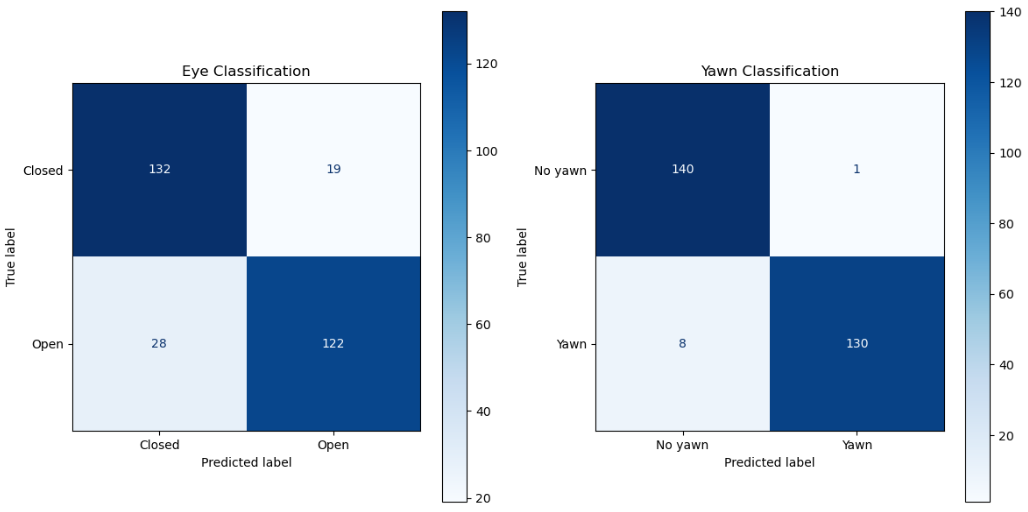
\includegraphics[width=14cm]{Images/SVM_cm.png}

\end{codebox}

\textbf{Interpretation\\}


Overall, the model excels at distinguishing between "yawn" and "no yawn," achieving high precision, recall, and F1-Score. It demonstrates high accuracy and balanced performance across most classes. However, some challenges remain in the eye-related classes, with precision for "closed" at 82\% and recall for "open" at 81\%. These issues should be monitored in future iterations to determine whether they represent persistent difficulties.

The macro-average metrics—91\% for precision, recall, and F1-Score—indicate that the model performs well across all classes without bias. Similarly, the weighted average confirms strong performance across the dataset, reflecting the balanced class distribution achieved during preprocessing.






\newpage

\subsection{Random Forest Classifier}

\bigskip

\textbf{Description\\}

\begin{itemize}
    \item \textbf{Objective:} The Random Forest classifier works by creating an ensemble of decision trees to classify images as "eyes opened" or "eyes closed." 
    It combines predictions from multiple decision trees to improve accuracy and reduce the risk of overfitting.
    Each decision tree is trained on a random subset of the data and features (bagging and feature sampling) to ensure diversity.

    \item \textbf{Input:} The Random Forest takes the image features as input. These features are the raw pixel values. Each feature is used to make binary decisions at the nodes of the decision trees.

    \item \textbf{Output:} The classifier outputs a probability score or a class label:
    \begin{itemize}
        \item \textbf{Probability Score:} For each image, the Random Forest outputs the proportion of trees voting for each class.
        \item \textbf{Class Label:} The final prediction is the class that receives the majority vote from all decision trees.
    \end{itemize}

    \item \textbf{Hyperparameters:}
    \begin{itemize}
        \item n estimators: The number of decision trees in the forest. Here, it is set to 100.
        \item Random state : Fixed seed for the random number generator. We used 42.
        \item Max depth : By default set to None, tree expands until all leaves contain only one class or until the number of samples in a node is less than min sample split (by default 2).
    \end{itemize}
    
   
\end{itemize}
\bigskip
\textbf{Code and outputs\\}
\begin{codebox}[RF Classifier]{Random Forest Classifier \texttt{Python}}
\begin{lstlisting}
from sklearn.ensemble import RandomForestClassifier
# Train Random Forest model
rf_model = RandomForestClassifier(n_estimators=100, random_state=42)
rf_model.fit(X_train, y_train)

# Predict on test data
y_pred_rf = rf_model.predict(X_test)

# Evaluate Random Forest performance
print("Random Forest Classification Report:")
print(classification_report(y_test, y_pred_rf))
print(f"Random Forest Accuracy: {accuracy_score(y_test, y_pred_rf):.2f}")
\end{lstlisting}
\end{codebox}


\begin{codebox}[OutputD]{ Random Forest Classification Report and Confusion Matrices}
\begin{lstlisting}
Random Forest Classification Report:
              precision    recall  f1-score   support

      Closed       0.92      0.88      0.90       151
        Open       0.89      0.92      0.90       150
     no_yawn       0.92      1.00      0.96       141
        yawn       1.00      0.92      0.96       138

    accuracy                           0.93       580
   macro avg       0.93      0.93      0.93       580
weighted avg       0.93      0.93      0.93       580

Random Forest Accuracy: 0.93
\end{lstlisting}

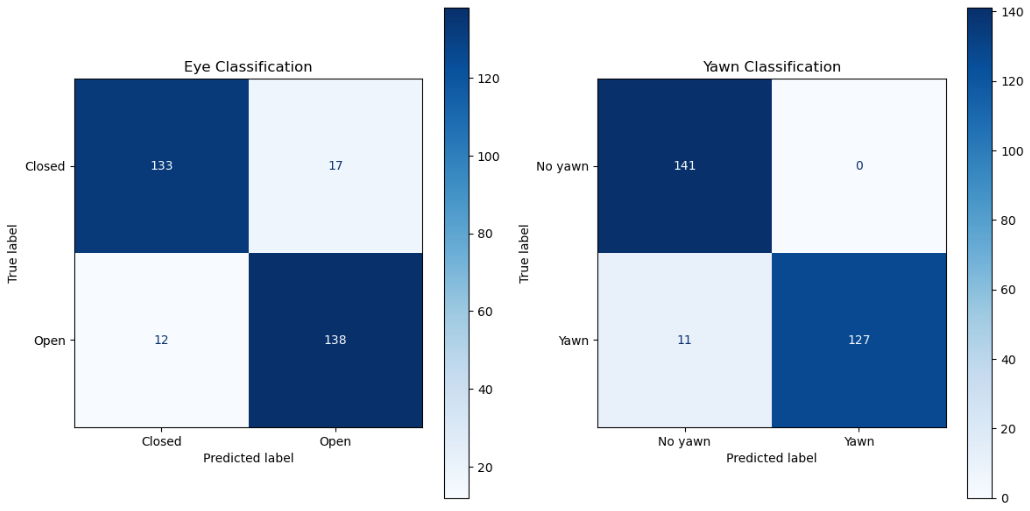
\includegraphics[width=14cm]{Images/RF_cm.png}

\end{codebox}

\textbf{Interpretation\\}

The accuracy of this model is better than the previous one.
According to the confusion matrix, the number of errors in labelization has reduced significantly.
The “open”/”closed” classes remain a bit difficult to labelize in comparison of the “yawn”, but it had made some progress. Note that this model tend to label a little bit more of “yawn” even if it implies more false negatives for the “no yawn” part.
F1 and recall scores underline that this model performs well across all classes without bias.

The Random Forest Classifier is slightly better for this dataset than the SVM with those hyperparameters. It has performed well for the eye with the “closed” and “open” class. But we need to also focus on the false negative result in the “yawn” class , and see if any particular features are causing confusion with “no yawn”.




\newpage

\subsection{Logistic Regression}

\bigskip

\textbf{Description\\}

\begin{itemize}
    \item \textbf{Objective:} Model the probability that a given image belongs to one of the two classes.
    It uses a logistic (sigmoid) function to map the linear combination of input features to a probability score between 0 and 1, which can then be thresholded to assign a class label.

    \item \textbf{Input:} The Logisitc Regression takes the image features as input. These features are the raw pixel values.Regression takes a vector of these features and applies a linear transformation (i.e., weighted sum) to calculate a score.

    \item \textbf{Output:} Logistic Regression outputs a probability score between 0 and 1. This score represents the likelihood that the image belongs to a particular class (e.g., the probability that the image is "eyes opened").

    \item \textbf{Hyperparameters:}
    \begin{itemize}
        \item max iter: Maximum number of iterations for the solver to converge. Here, it is set to 1000.
        \item Random state : Fixed seed for the random number generator. We used 42.
        \item Solver : lbfgs by default.
    \end{itemize}
   
\end{itemize}
\bigskip
\bigskip
\textbf{Code and outputs\\}
\begin{codebox}[LR Classifier]{Logistic Regression \texttt{Python}}
\begin{lstlisting}
from sklearn.linear_model import LogisticRegression

# Train Logistic Regression model
lr_model = LogisticRegression(max_iter=1000, random_state=42)
lr_model.fit(X_train, y_train)

# Predict on test data
y_pred_lr = lr_model.predict(X_test)

# Evaluate Logistic Regression performance
print("Logistic Regression Classification Report:")
print(classification_report(y_test, y_pred_lr))
print(f"Logistic Regression Accuracy: {accuracy_score(y_test, y_pred_lr):.2f}")
\end{lstlisting}
\end{codebox}


\begin{codebox}[OutputE]{ Logistic Regression Report and Confusion Matrices}
\begin{lstlisting}
Logistic Regression Classification Report:
              precision    recall  f1-score   support

      Closed       0.85      0.92      0.88       151
        Open       0.92      0.83      0.87       150
     no_yawn       0.93      0.99      0.96       141
        yawn       0.99      0.93      0.96       138

    accuracy                           0.92       580
   macro avg       0.92      0.92      0.92       580
weighted avg       0.92      0.92      0.92       580

Logistic Regression Accuracy: 0.92
\end{lstlisting}

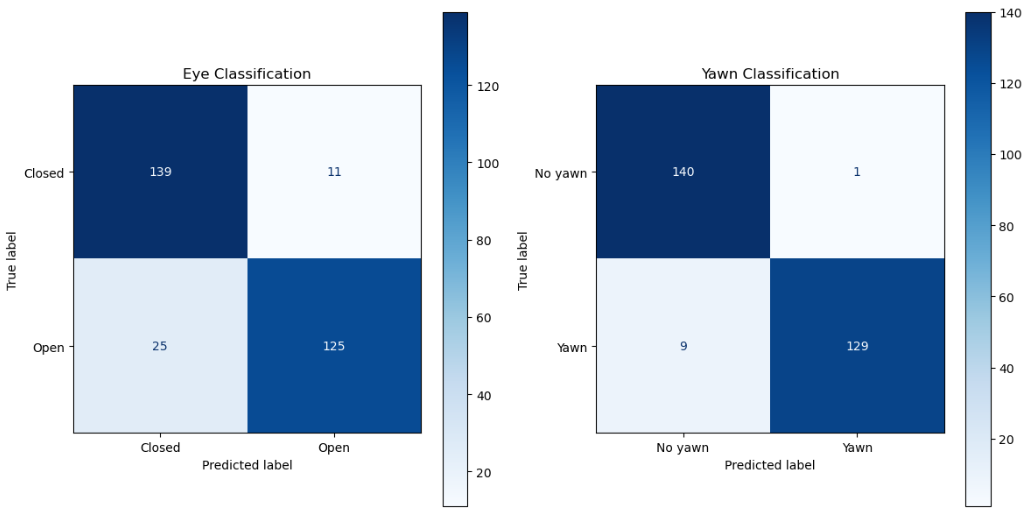
\includegraphics[width=14cm]{Images/LR_cm.png}

\end{codebox}

\textbf{Interpretation\\}

The overall accuracy for Logistic Regression is high, matching the Random Forest model's performance and slightly better than the SVM model. We lost a lot of precision in the “close” class -almost the double of errors- but overall made some progress for the other class, gaining some precision on the “open” class and in the “no yawn”. The macro average and the weighted average is almost the same as the other model.
So, Logistic Regression offers competitive performance with some trade-offs compared to the other models.

%---------------------------------------
\newpage

\section{Testing our models' Robustness}

The problem with training on datasets found online, especially on Kaggle, is the similarity the data may exhibit. This can lead to models that overfit or underfit the data we provide.\\\\
To avoid this issue, we gathered what we referred to as "Real-Life Data." Specifically, we took pictures ourselves in the real world (as opposed to sourcing them online) to test our models. These images featured a variety of shapes, new faces, and different eye conditions for testing.
\\\\

The results were promising out of 32 images we got:
\begin{itemize}
    \item 97\% of correctly labeled images by the SVM.
    \item 97\% of correctly labeled images by the Random Forest.
    \item 100\% of correctly labeled images by the Linear Regression.\\\\
\end{itemize}

Although this outcome can be partly attributed to the relatively small size of our Real-Life Dataset, it still highlights the robustness and consistency of our models.
\\\\\\
\textbf{Notes:}
\begin{itemize}
    \item We limited our tests to labeling images as "eyes open" or "eyes closed. This ensured the used pictures to be centered around the eyes of our volunteers, ensuring some kind of privacy regarding their identities.
    \item The "Real-Life Data" isn't available on the project's GitHub, or anywhere else, for privacy matters.
\end{itemize} 


%---------------------------------------
\newpage

\section{Going Deeper}

\subsection{Implementing a Convolutional Neural Network}

In this section, we detail the implementation of a Convolutional Neural Network (CNN) for classifying images in our dataset. 
CNNs are a type of deep learning model particularly well-suited for image processing tasks. They are designed to automatically 
and adaptively learn spatial hierarchies of features, from edges to shapes to complex structures, through the use of 
convolutional and pooling layers.

We used the Keras library to construct and train our model. Below, we present the architecture and the results of the 
training process.

\subsubsection{CNN Architecture}

The architecture of our CNN consists of convolutional layers to extract spatial features, followed by pooling layers 
to reduce dimensionality. After these, fully connected (dense) layers are used for classification. The network ends with a 
softmax layer, which outputs probabilities for each class. The Python code below defines the CNN architecture


\begin{codebox}[CNN architecture]{CNN Architecture definition \texttt{Python}}
\begin{lstlisting}
model = Sequential()

# Convolutional layer 1
model.add(Conv2D(32, (3, 3), activation="selu", input_shape=(64,64,1)))
model.add(MaxPooling2D(2, 2))

# Convolutional layer 2
model.add(Conv2D(32, (3, 3), activation="selu"))
model.add(MaxPooling2D(2, 2))

# Convolutional layer 3
model.add(Flatten())
model.add(Dropout(0.5))

# Convolutional layer 4
model.add(Dense(64, activation="relu"))
model.add(Dense(4, activation="softmax"))

# Compilation
model.compile(loss="categorical_crossentropy", metrics=["accuracy"], optimizer="adam")

model.summary()
\end{lstlisting}
\end{codebox}

\textbf{Explanation of the Architecture}

\begin{enumerate}
    \item \textbf{Convolutional Layers: }The first two layers are convolutional layers with 32 filters of size 3x3. The `selu` 
    activation function is used, which helps with self-normalizing activations. These layers capture spatial features 
    from the input images.
    \item \textbf{Max Pooling Layers: }Each convolutional layer is followed by a max pooling layer with a pool size of 2x2. 
    Pooling reduces the spatial dimensions, making the computation more efficient while retaining important features.
    \item \textbf{Flattening and Dropout: }The output of the last pooling layer is flattened into a one-dimensional vector, 
    transforming the spatial data into a format suitable for fully connected layers. A dropout layer with a rate of 0.5 is 
    added to reduce overfitting by randomly deactivating 50\% of the neurons during training, ensuring that the model 
    generalizes well to new data.
\end{enumerate}





\newpage

\subsubsection{CNN Results and Performance Evaluation}

After training the CNN on our dataset, we evaluated its performance using metrics such as precision, recall, F1-score, 
and accuracy. The results of the evaluation, including a classification report and a confusion matrix, are presented below.

\begin{codebox}[OutputG]{ CNN Results after being trained on our dataset}
    \begin{lstlisting}
    Model: "sequential_11"
    19/19 [==============================] - 0s 8ms/step
CNN Classification Report:
            precision    recall  f1-score   support

        0       0.97      0.99      0.98       151
        1       0.93      0.97      0.95       141
        2       0.97      0.92      0.94       149
        3       0.99      0.97      0.98       139

accuracy                            0.96       580
macro avg       0.96      0.96      0.96       580
weighted avg    0.96      0.96      0.96       580

CNN Accuracy: 0.96
    \end{lstlisting}

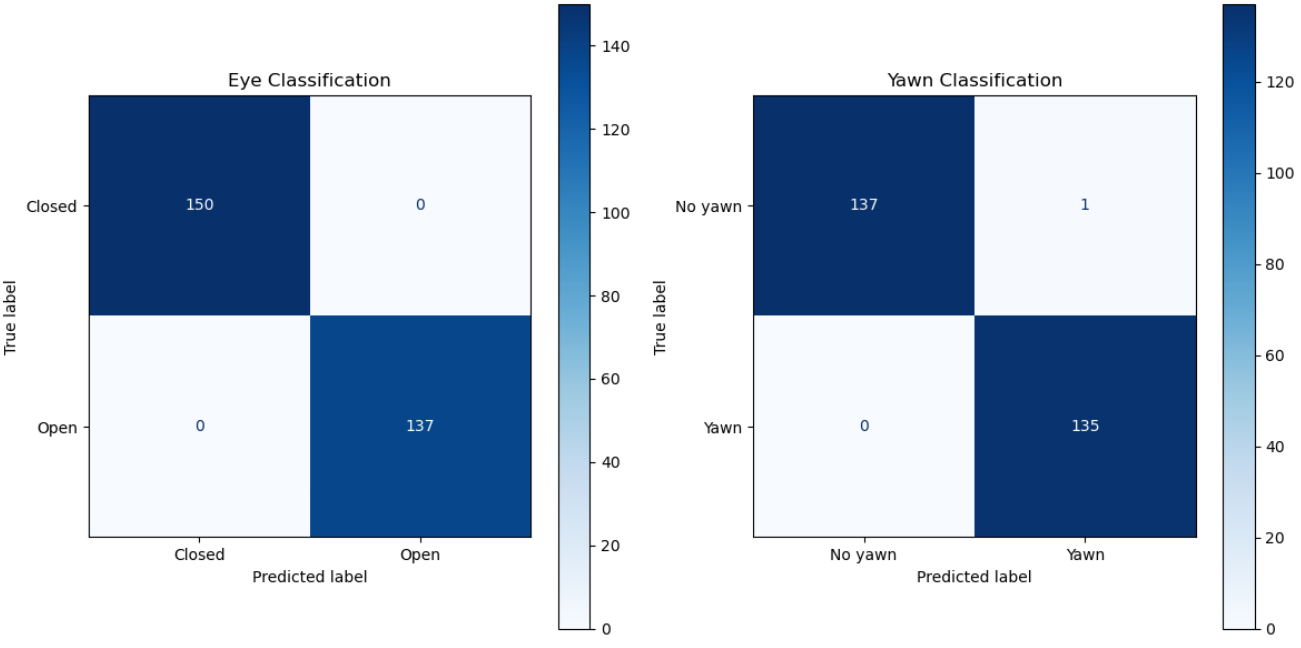
\includegraphics[width=14cm]{Images/CNN_cm.png}

\end{codebox}
\newpage
\textbf{Explanation of Metrics:}\\
\begin{itemize}
    \item \textbf{Precision:} Precision indicates the percentage of true positive predictions out of all positive 
    predictions made by the model. In our case, precision values range between 93\% and 99\%, demonstrating that the 
    model produces very few false positives.
    \item \textbf{Recall:} Recall measures the percentage of actual positive samples that were correctly predicted. 
    The recall values for the four classes range from 92\% to 99\%, indicating the model effectively identifies positive 
    samples.
    \item \textbf{F1-Score:} The F1-score is the harmonic mean of precision and recall, providing a balanced measure of 
    the model's performance. Scores close to 1 across all classes show that the model performs consistently well.
    \item \textbf{Accuracy:} The overall accuracy of the model is 96\%, indicating that it correctly classified 96\% of the 
    samples in the test set.\\
\end{itemize}

\textbf{Confusion Matrix}\\

The confusion matrix provides a detailed breakdown of the model's performance on each class by comparing the predicted and 
actual labels. It highlights where the model makes errors and gives insight into which classes are more challenging for the 
network to distinguish.\\

\textbf{Insights from the Confusion Matrix:}\\
\begin{itemize}
    \item Most samples are classified correctly, as evidenced by the high values along the diagonal.
    \item Misclassifications are minimal, with a few cases where the model confuses certain classes. 
    These errors might be due to class similarity or limitations in the dataset.\\
\end{itemize}

\textbf{Conclusion:}\\

The CNN achieves excellent performance with an overall accuracy of 96\%. The high precision, recall, 
and F1-scores across all classes indicate that the model generalizes well to unseen data. While there are minor 
misclassifications, these can potentially be addressed by augmenting the dataset, fine-tuning the model architecture, 
or employing advanced techniques such as transfer learning.


%---------------------------------------

\insererbiblio
\end{document}